\appendix
\chapter{Appendices}
% \addcontentsline{toc}{chapter}{Appendices}

\section{Metrics}
\label{append:metrics}

The following information was retrieved from the Supplementary Material provide by Castro et al. \cite{castro2021mico}. 

A \textbf{metric} \(d\) on a set \(X\) is a function \(d : X \times X \to [0, \infty)\) respecting the following axioms for any \(x, y, z \in X\):

\begin{enumerate}
    \item \textbf{Identity of indiscernibles:} \(d(x, y) = 0 \iff x = y\);
    \item \textbf{Symmetry:} \(d(x, y) = d(y, x)\);
    \item \textbf{Triangle inequality:} \(d(x, y) \leq d(x, z) + d(z, y)\).
\end{enumerate}

A \textbf{pseudometric} is similar, but the "identity of indiscernibles" axiom is weakened:

\begin{enumerate}
    \item \(x = y \implies d(x, y) = 0\);
    \item \(d(x, y) = d(y, x)\);
    \item \(d(x, y) \leq d(x, z) + d(z, y)\).
\end{enumerate}

Note that the weakened first condition \emph{does} allow one to have \(d(x, y) = 0\) when \(x \neq y\).

A \textbf{(pseudo)metric space} \((X, d)\) is defined as a set \(X\) together with a (pseudo)metric \(d\) defined on \(X\).

A \textbf{diffuse metric} is similar to as pseudometri, but the 'identity of indiscernibles' axiom is weakened even more:

\begin{enumerate}
    \item \(d(x, y) \geq 0\) for any $x, y \in X$;
    \item \(d(x, y) = d(y, x)\);
    \item \(d(x, y) \leq d(x, z) + d(z, y)\).
\end{enumerate}

Note that the weakened first condition \emph{does} allow one to have self-distance greater than zero $d(x,x) > 0$.

\section{Algorithm: DQN with Matching under Independent Couplings (MICo)}
\label{append:dqn_mico}

\begin{algorithm}[H]
\caption{DQN with Matching under Independent Couplings (MICo)}
\label{algorithm:dqn_mico}
\begin{algorithmic}[1]
\State \textbf{Input:} minibatch $k$, step-size $\eta$, replay period $K$ and size $N$, budget $T$ (total steps).
\State \textbf{Initialize} action-value function $Q$ with random weights $\xi$, $\omega$
\State \textbf{Initialize} target action-value function $Q^-$ with weights $\{\bar{\xi},\bar{\omega}\} \leftarrow \{\xi, \omega\}$
\State \textbf{Initialize} replay memory $\mathcal{D} = \emptyset$ with capacity $N$%$\Delta_{\{\xi, \omega\}} = 0$, $\Delta_\omega = 0$, $p_1 = 1$
% \State Observe $s_0$ and choose $a_0 \sim \pi^\epsilon_\theta(s_0)$ 
\For{$t = 1$ to $T$}
    \State Observe $s_t$
    \State Choose action $a_t \sim \pi^\epsilon_\theta(s_t)$
    \State Execute action $a_t$ and observe $r_t$ and $s_{t+1}$
    \State Store transition $(s_t, a_t, r_t, s_{t+1})$ in $\mathcal{D}$
    \If{$t \equiv 0 \mod K$}
        % \For{$j = 1$ to $k$}
        \State Sample minibatch $B \sim \text{Uniform}(\mathcal{D})$ of transitions $e_j$        % \State Compute importance-sampling weight $w_j = \left( N \cdot P(j) \right)^{-\beta} / \max_i w_i$
        \State Set $y_j = 
        \begin{cases} 
            r_j & \text{for terminal } s_{j+1}\\
            r_j + \gamma \max_{a'} Q^-(s_{j+1}, a'; \{\bar{\xi},\bar{\omega}\}) & \text{otherwise}
        \end{cases}$
        \State Compute TD-error $\delta_j = y_j - Q(s_{j}, a_{j}; \{\xi, \omega\})$, and loss $\mathcal{L}_{\text{TD}} = \delta_j^2 $
        \State Squarify minibatch $B$ to get transition pairs $\left\langle x, r_x, x^{\prime}\right\rangle,\left\langle y, r_y, y^{\prime}\right\rangle$ 
        \State Compute MICo loss $\mathcal{L}_{\text{MICo}} = \left(T_{\bar{\omega}}^U\left(r_x, x^{\prime}, r_y, y^{\prime}\right)-U_\omega(x, y)\right)^2$
        \State Compute total loss $\mathcal{L}_\alpha(\xi, \omega) = (1 - \alpha) \mathcal{L}_{\text{TD}}(\xi, \omega) + \alpha \mathcal{L}_{\text{MICo}}(\omega)$
        \State Perform a gradient descent step on $\mathcal{L}_\alpha(\xi, \omega)$
        % \State Update transition priority $p_j \leftarrow (1 - \mu) |\delta_j| + \mu U_\omega(s_j,s_{j+1}) + \epsilon$
        \State Every C optimizing steps update $\{\bar{\xi},\bar{\omega}\} \leftarrow \{\xi, \omega\}$
        

        
        % \State Accumulate weight-change $\Delta_{\{\xi, \omega\}} \leftarrow \Delta_{\{\xi, \omega\}} + w_j \cdot \delta_j \cdot \nabla_\theta Q(s_{j}, a_{j})$
        % \State Compute bisimulation distance error $\sigma_j = T_{\bar{\omega}}^U\left(r_x, x^{\prime}, r_y, y^{\prime}\right)-U_\omega(x, y)$
        %  \State Accumulate weight-change $\Delta_{\omega} \leftarrow \Delta_{\omega} + w_j \cdot \sigma_j \cdot \nabla_\omega U_\omega(s_{i}, a_{j})$   

        % \EndFor
        % \State Update weights $\theta \leftarrow \theta + \eta \cdot \Delta$, reset $\Delta = 0$
    \EndIf
\EndFor
\end{algorithmic}
\end{algorithm}

\section{Distance between Priority Sampling Distributions}

% Given the sampling distribution of priorities pi(·) from the experience buffer and
% the corresponding ideal distribution p
% ∗
% i
% (·) (theoretically achieved when all state
% space priorities are updated at each time step7
% ), 1) the on-policy weighting is
% given by P31
% j=1 w
% π
% (sj )|pi(sj ) − p
% ∗
% i
% (sj )|, i ∈ {1, 2}, and 2) the uniform weighting is
% 1
% 31
% P31
% j=1 |pi(sj ) − p
% ∗
% i
% (sj )|, i ∈ {1, 2}, where p1 corresponds to the PER method and
% p2 corresponds to the BPER method. A more detailed explanation of this procedure
% is provided in the Appendix ??.

\section{Hyperparameters Setting}
\label{append:hyperparameters}

\begin{table}[H]
\centering

\hspace*{-1cm}
\begin{tabular}{@{} lccccc @{}}
\toprule
& \textbf{Hyperparameter} & {\footnotesize\textbf{DQN}} & {\footnotesize \textbf{DQN PER}} & {\footnotesize\textbf{DQN MICo}} & {\footnotesize\textbf{DQN BPER}} \\ 
\midrule

\multirow{8}{*}{\textbf{Collector}} 
& Total Budget & 100,000 & 100,000 & 100,000 & 100,000 \\ 
& Replay Period & 128 & 128 & 128 & 128 \\ 
& Eps Start & 0.1 & 0.1 & 0.1 & 0.1 \\ 
& Eps End & 0.005 & 0.005 & 0.005 & 0.005 \\ 
& Eps Annealing Frames & 520,000 & 520,000 & 520,000 & 520,000 \\ 
& Init Random Frames & 200 & 200 & 200 & 200 \\ 
& Frame Stack & 1 & 1 & 1 & 1 \\
& Frame Skip & 1 & 1 & 1 & 1 \\ 
\midrule

\multirow{5}{*}{\textbf{Policy}} 
& CNN Net (Cells) & [32, 64, 64] & [32, 64, 64] & [32, 64, 64] & [32, 64, 64] \\ 
& Kernel Sizes & [8, 4, 3] & [8, 4, 3] & [8, 4, 3] & [8, 4, 3] \\ 
& Strides & [4, 2, 1] & [4, 2, 1] & [4, 2, 1] & [4, 2, 1] \\ 
& MLP Net (Cells) & [64, 64] & [64, 64] & [64, 64] & [64, 64] \\ 
& Activation & ReLU & ReLU & ReLU & ReLU \\ 
\midrule

\multirow{5}{*}{\textbf{Buffer}} 
& Buffer Size & 100,000 & 100,000 & 100,000 & 100,000 \\ 
& Batch Size & 256 & 256 & 256 & 256 \\ 
& Alpha & -- & 0.6 & -- & 0.6 \\ 
& Beta & -- & 0.4 & -- & 0.4 \\ 
& Priority Weight & -- & -- & 1.0 & 1.0 \\ 
\midrule

\multirow{4}{*}{\textbf{Optim}} 
& Learning Rate & 0.0015 & 0.0015 & 0.0015 & 0.0015 \\ 
& Max Grad Norm & 10 & 10 & 10 & 10 \\ 
& Weight Decay & 0.00001 & 0.00001 & 0.00001 & 0.00001 \\ 
& Eps & 1.5e-4 & 1.5e-4 & 1.5e-4 & 1.5e-4 \\ 
\midrule

\multirow{6}{*}{\textbf{Loss}} 
& Gamma & 0.99 & 0.99 & 0.99 & 0.99 \\ 
& MICO Weight & -- & -- & 0.01 & 0.01 \\ 
& MICO Beta & -- & -- & 0.1 & 0.1 \\ 
& MICO Gamma & -- & -- & 0.99 & 0.99 \\ 
& Hard Update Freq & 50 & 50 & 50 & 50 \\ 
& Num Updates & 1 & 1 & 1 & 1 \\ 
\bottomrule

\end{tabular}
\caption[Hyperparameter Configurations for Grid World]{\textbf{Hyperparameter Configurations for Grid World.} This configuration was consistently used among different independent runs, where the setting for DQN BPER works for both BPERcn and BPERaa.}
\end{table}

\begin{table}[H]
\centering

\hspace*{-1cm}
\begin{tabular}{@{} lccccc @{}}
\toprule
& \textbf{Hyperparameter} & {\footnotesize\textbf{DQN}} & {\footnotesize \textbf{DQN PER}} & {\footnotesize\textbf{DQN MICo}} & {\footnotesize\textbf{DQN BPER}} \\ 
\midrule

\multirow{8}{*}{\textbf{Collector}} 
& Total Budget & 1,000,064 & 1,000,064 & 1,000,064 & 1,000,064 \\ 
& Replay Period & 128 & 128 & 128 & 128 \\ 
& Eps Start & 0.5 & 0.5 & 0.5 & 0.5 \\ 
& Eps End & 0.005 & 0.005 & 0.005 & 0.005 \\ 
& Eps Annealing Frames & 520,000 & 520,000 & 520,000 & 520,000 \\ 
& Init Random Frames & 20,000 & 20,000 & 20,000 & 20,000 \\ 
& Frame Stack & 4 & 4 & 4 & 4 \\
& Frame Skip & 4 & 4 & 4 & 4 \\ 
\midrule

\multirow{5}{*}{\textbf{Policy}} 
& CNN Net (Cells) & [32, 64, 64] & [32, 64, 64] & [32, 64, 64] & [32, 64, 64] \\ 
& Kernel Sizes & [8, 4, 3] & [8, 4, 3] & [8, 4, 3] & [8, 4, 3] \\ 
& Strides & [4, 2, 1] & [4, 2, 1] & [4, 2, 1] & [4, 2, 1] \\ 
& MLP Net (Cells) & [64, 64] & [64, 64] & [64, 64] & [64, 64] \\ 
& Activation & ReLU & ReLU & ReLU & ReLU \\ 
\midrule

\multirow{5}{*}{\textbf{Buffer}} 
& Buffer Size & 100,000 & 100,000 & 100,000 & 100,000 \\ 
& Batch Size & 256 & 256 & 256 & 256 \\ 
& Alpha & -- & 0.6 & -- & 0.6 \\ 
& Beta & -- & 0.4 & -- & 0.4 \\ 
& Priority Weight & -- & -- & 1.0 & 1.0 \\ 
\midrule

\multirow{4}{*}{\textbf{Optim}} 
& Learning Rate & 0.0015 & 0.0015 & 0.0015 & 0.0015 \\ 
& Max Grad Norm & 10 & 10 & 10 & 10 \\ 
& Weight Decay & 0.00001 & 0.00001 & 0.00001 & 0.00001 \\ 
& Eps & 1.5e-4 & 1.5e-4 & 1.5e-4 & 1.5e-4 \\ 
\midrule

\multirow{6}{*}{\textbf{Loss}} 
& Gamma & 0.99 & 0.99 & 0.99 & 0.99 \\ 
& MICO Weight & -- & -- & 0.01 & 0.01 \\ 
& MICO Beta & -- & -- & 0.1 & 0.1 \\ 
& MICO Gamma & -- & -- & 0.99 & 0.99 \\ 
& Hard Update Freq & 50 & 50 & 50 & 50 \\ 
& Num Updates & 1 & 1 & 1 & 1 \\ 
\bottomrule

\end{tabular}
\caption[Hyperparameter Configurations for Other Environments]{\textbf{Hyperparameter Configurations for Other Environments.} This configuration was consistently applied across the MountainCar, CartPole, Acrobot, and LunarLander environments for each independent run. The settings for DQN BPER are applicable to both BPERcn and BPERaa. The priority weight configuration was adjusted as described in the results.}
\end{table}


\section{Priority Weight Sweep Results}
\label{append:priority_weight_sweep}

\begin{figure}[H]
    \centering
    \begin{subfigure}{0.45\textwidth}
    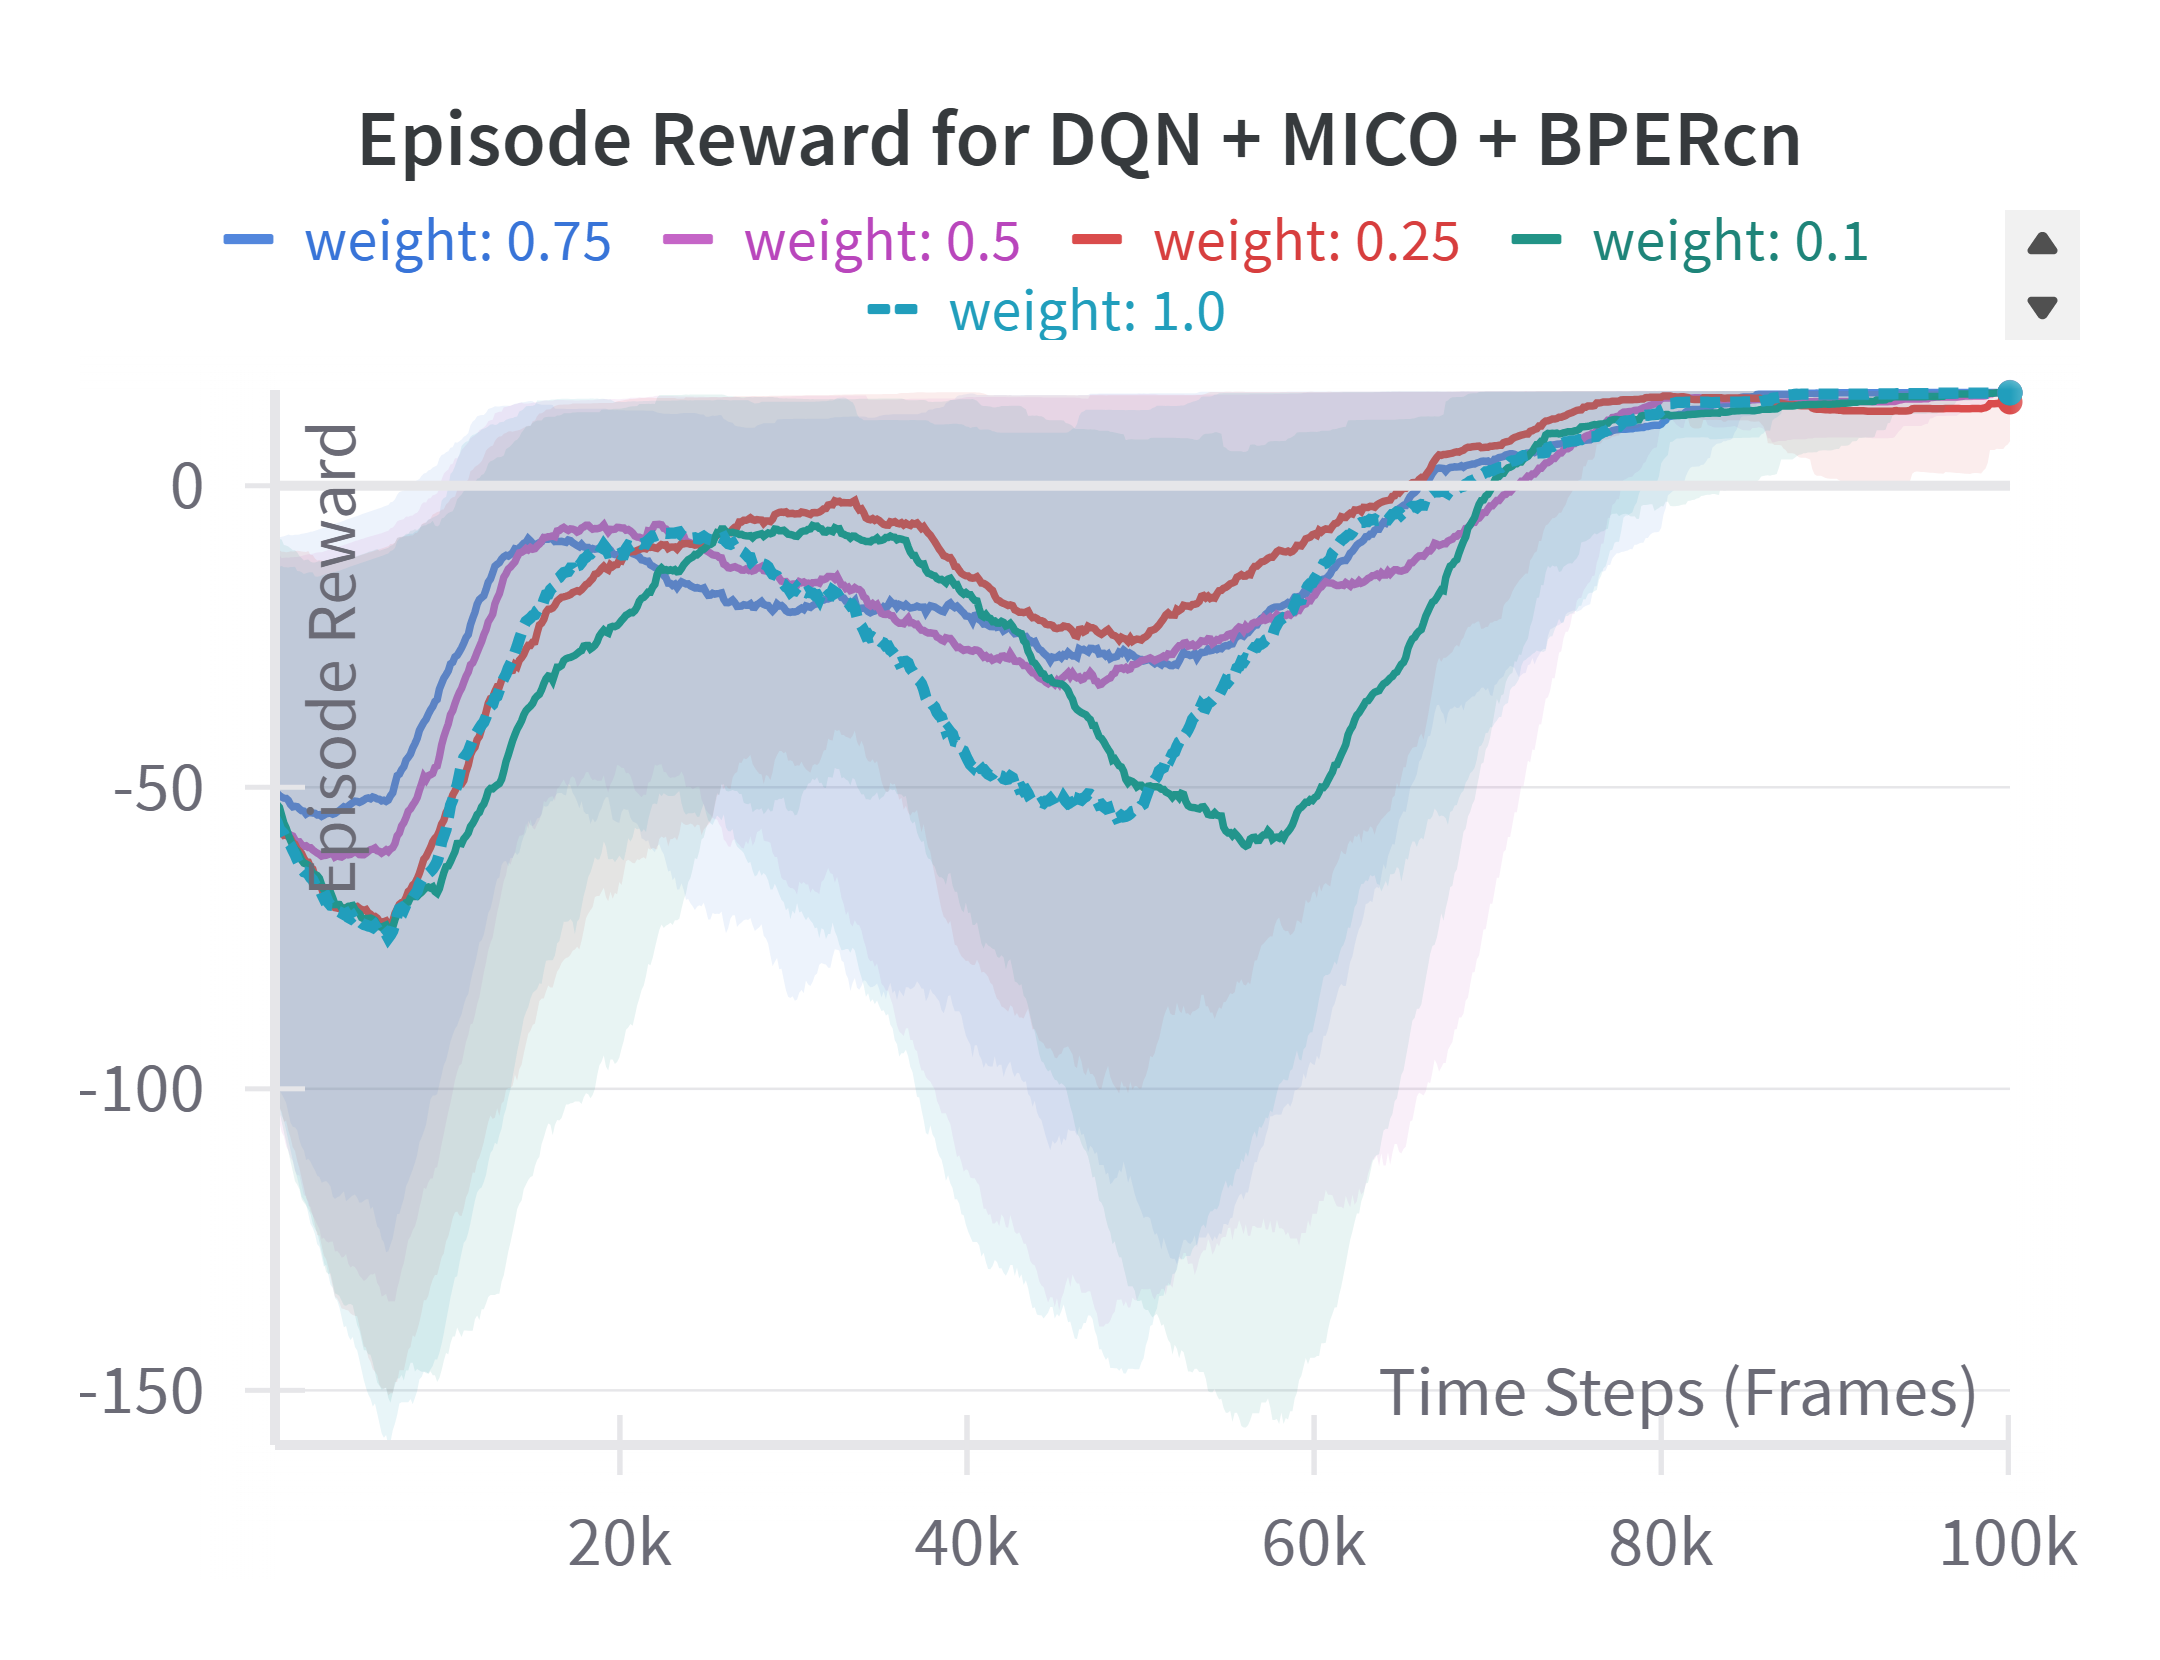
\includegraphics[width=\linewidth]{Results/grid_world/sweep_bpercn_grid_world.png}
        \caption{Sweep BPERcn}
        \label{fig:sweep_bpercn_grid_world}
    \end{subfigure}
    \hfill
    \begin{subfigure}{0.45\textwidth}
        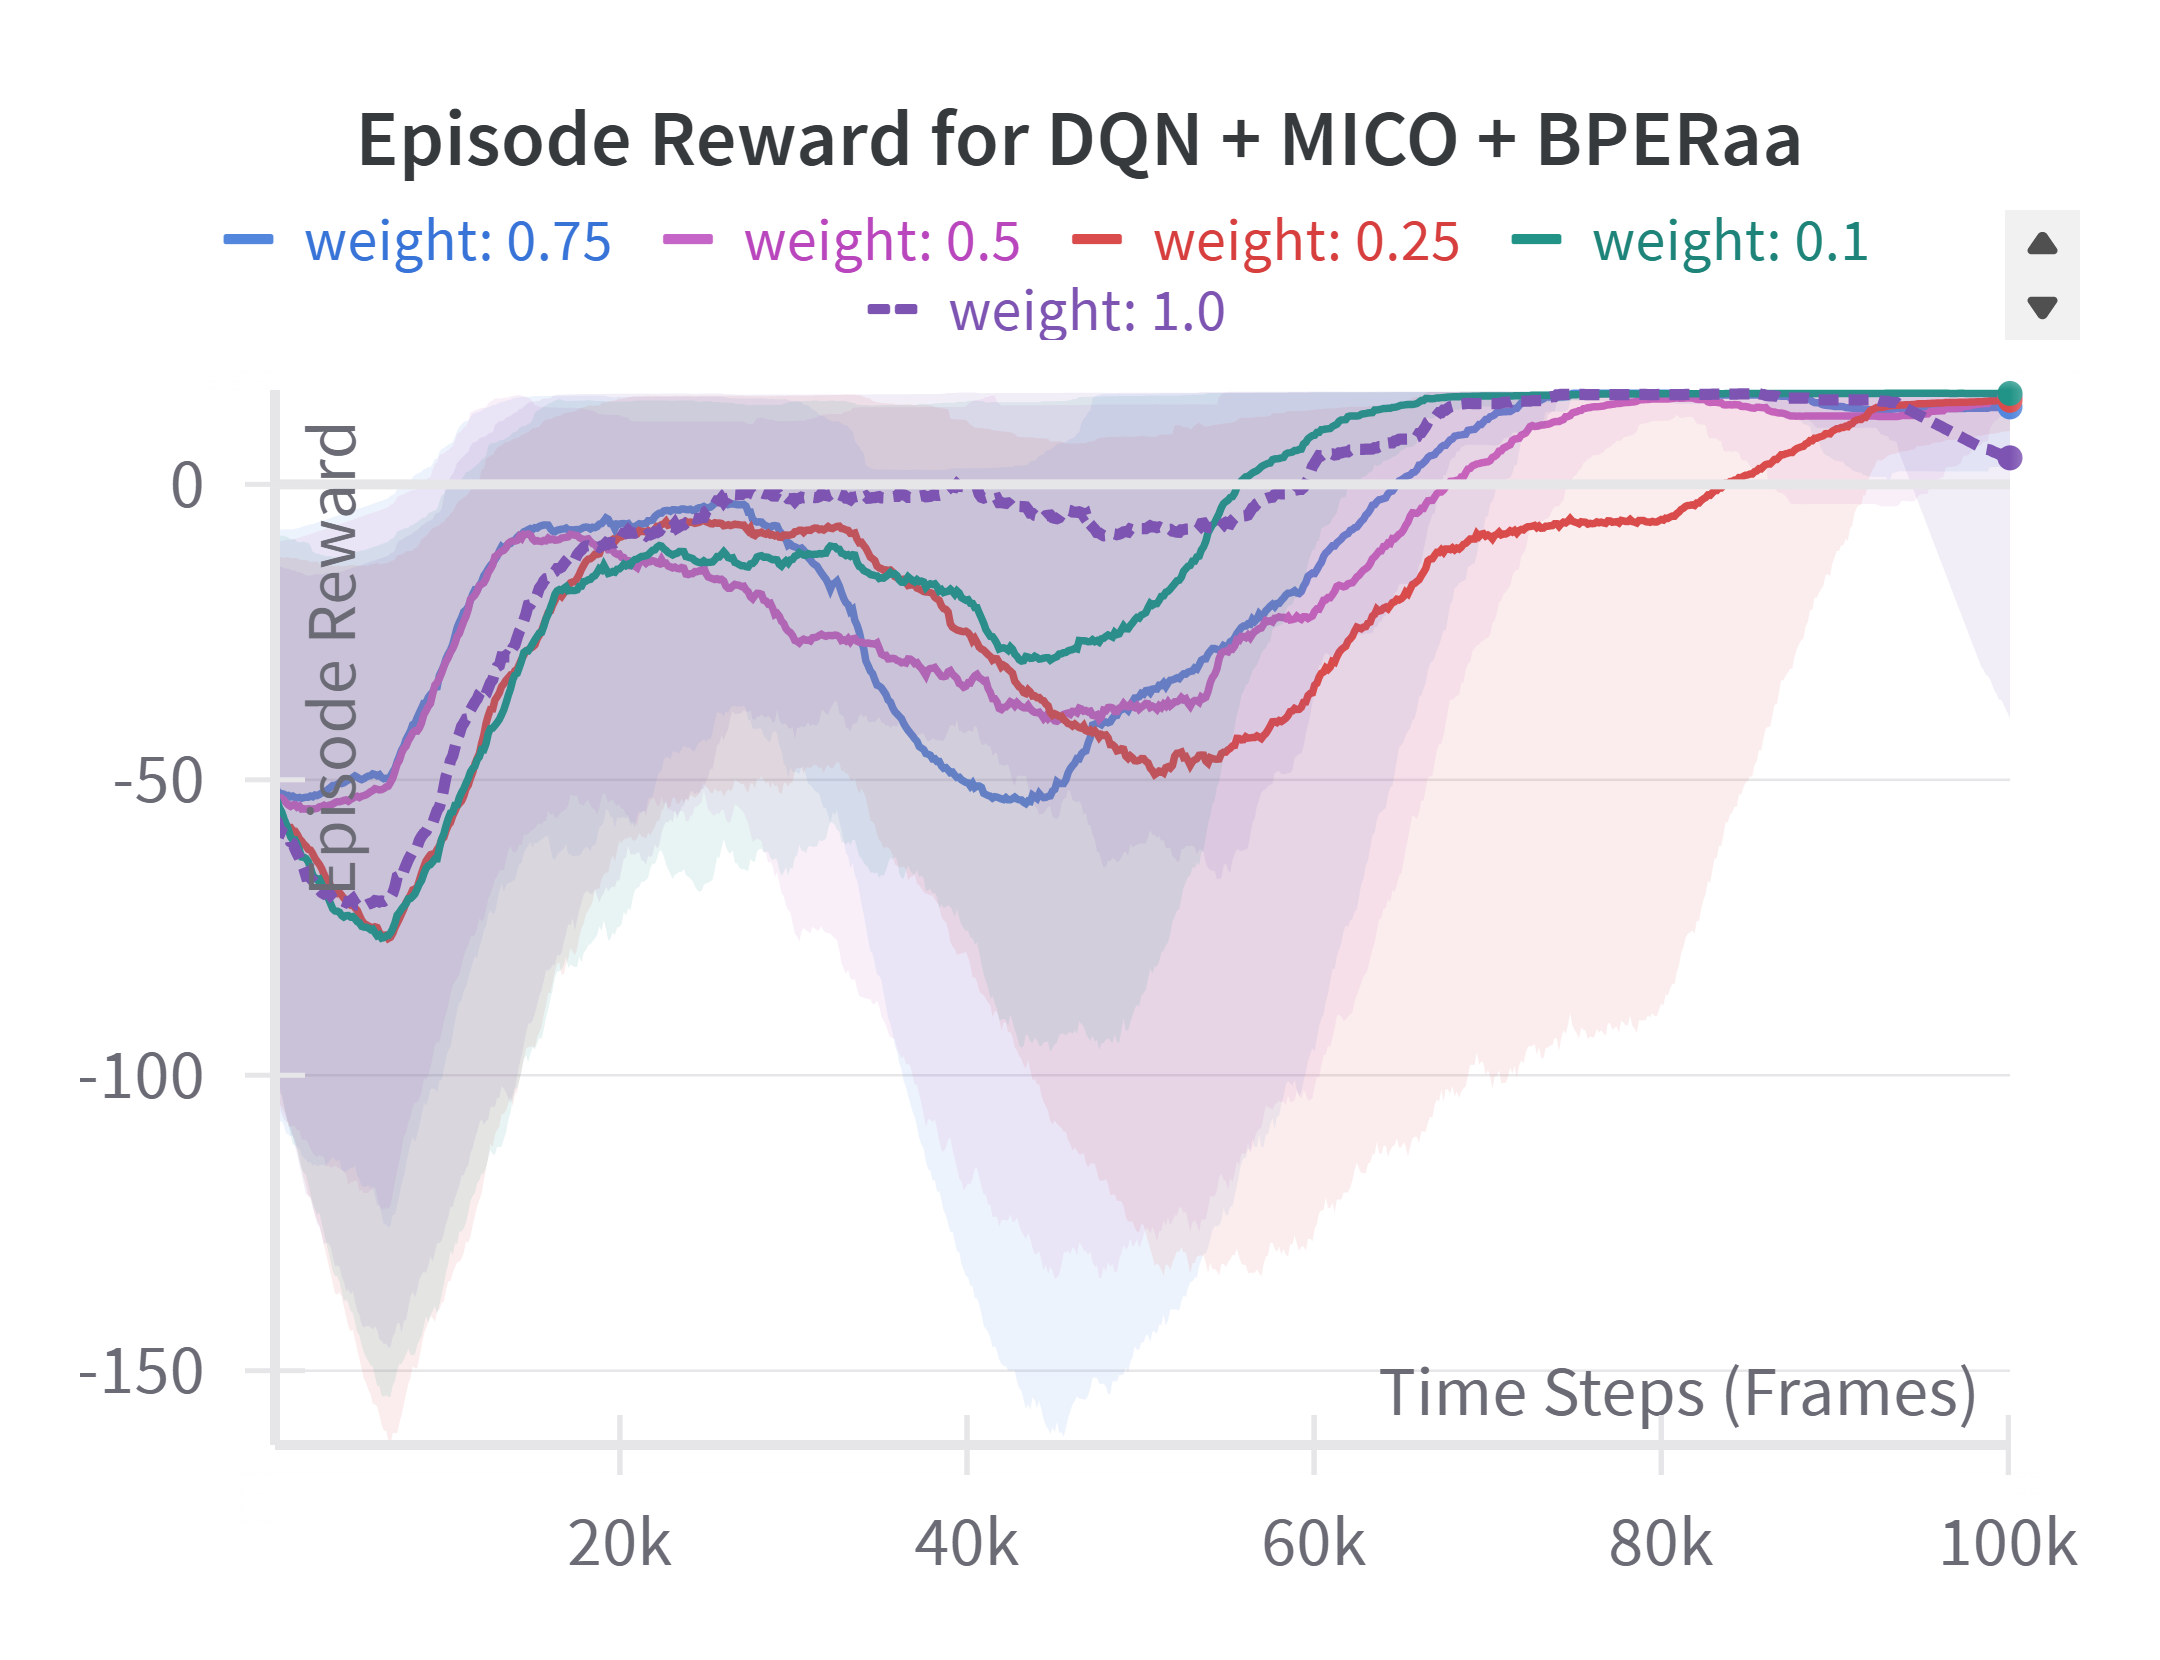
\includegraphics[width=\linewidth]{Results/grid_world/sweep_bperaa_grid_world.png}
        \caption{Sweep BPERcn}
        \label{fig:sweep_bperaa_grid_world}
    \end{subfigure}
    \caption[Priority Weight Sweep in Grid World]{\textbf{Priority Weight Sweep in Grid World.} TODO}
    \label{fig:sweep_methods_grid_world}
\end{figure}

\section{Mountain Car and CartPole with Priority Weight 1.0}
\label{append:results_priority_weight_1_0}
\begin{figure}[H]
    \centering
    \begin{subfigure}{0.45\textwidth}
    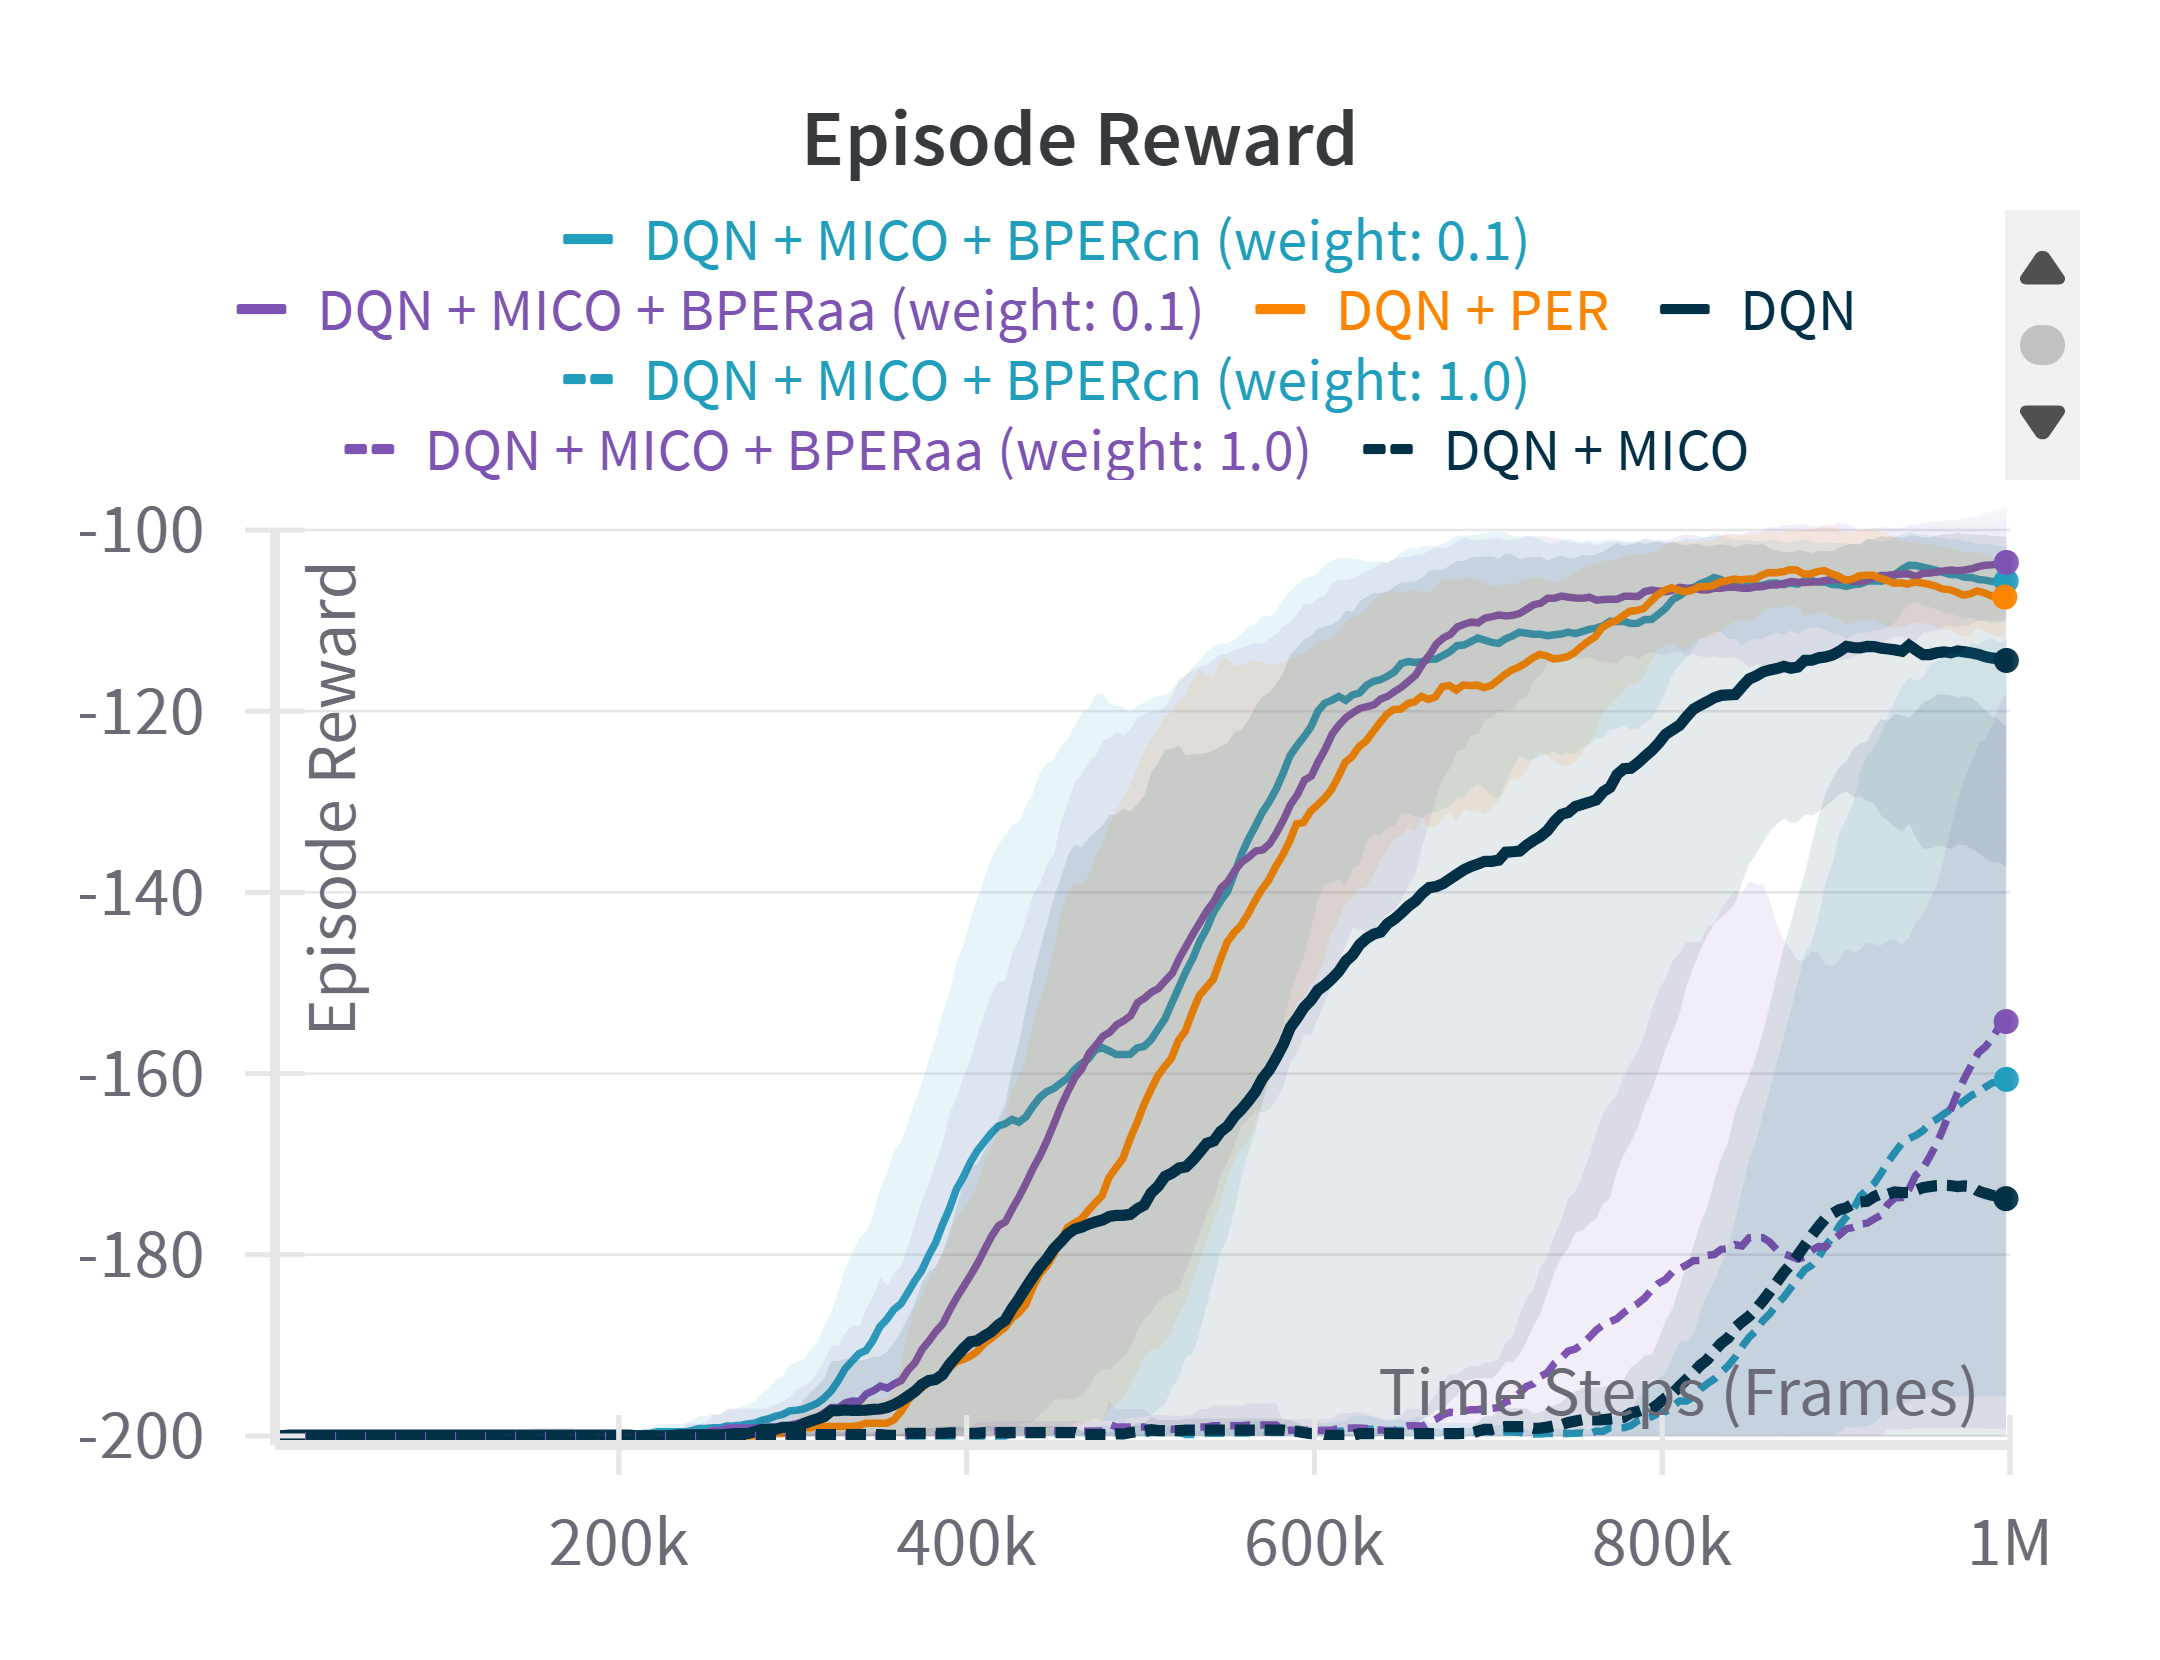
\includegraphics[width=\linewidth]{Results/general_results/return_mountain_car_weigh_1.png}
        \caption{Mountain Car}
        \label{fig:return_mountain_car_weigh_1}
    \end{subfigure}
    \hfill
    \begin{subfigure}{0.45\textwidth}
        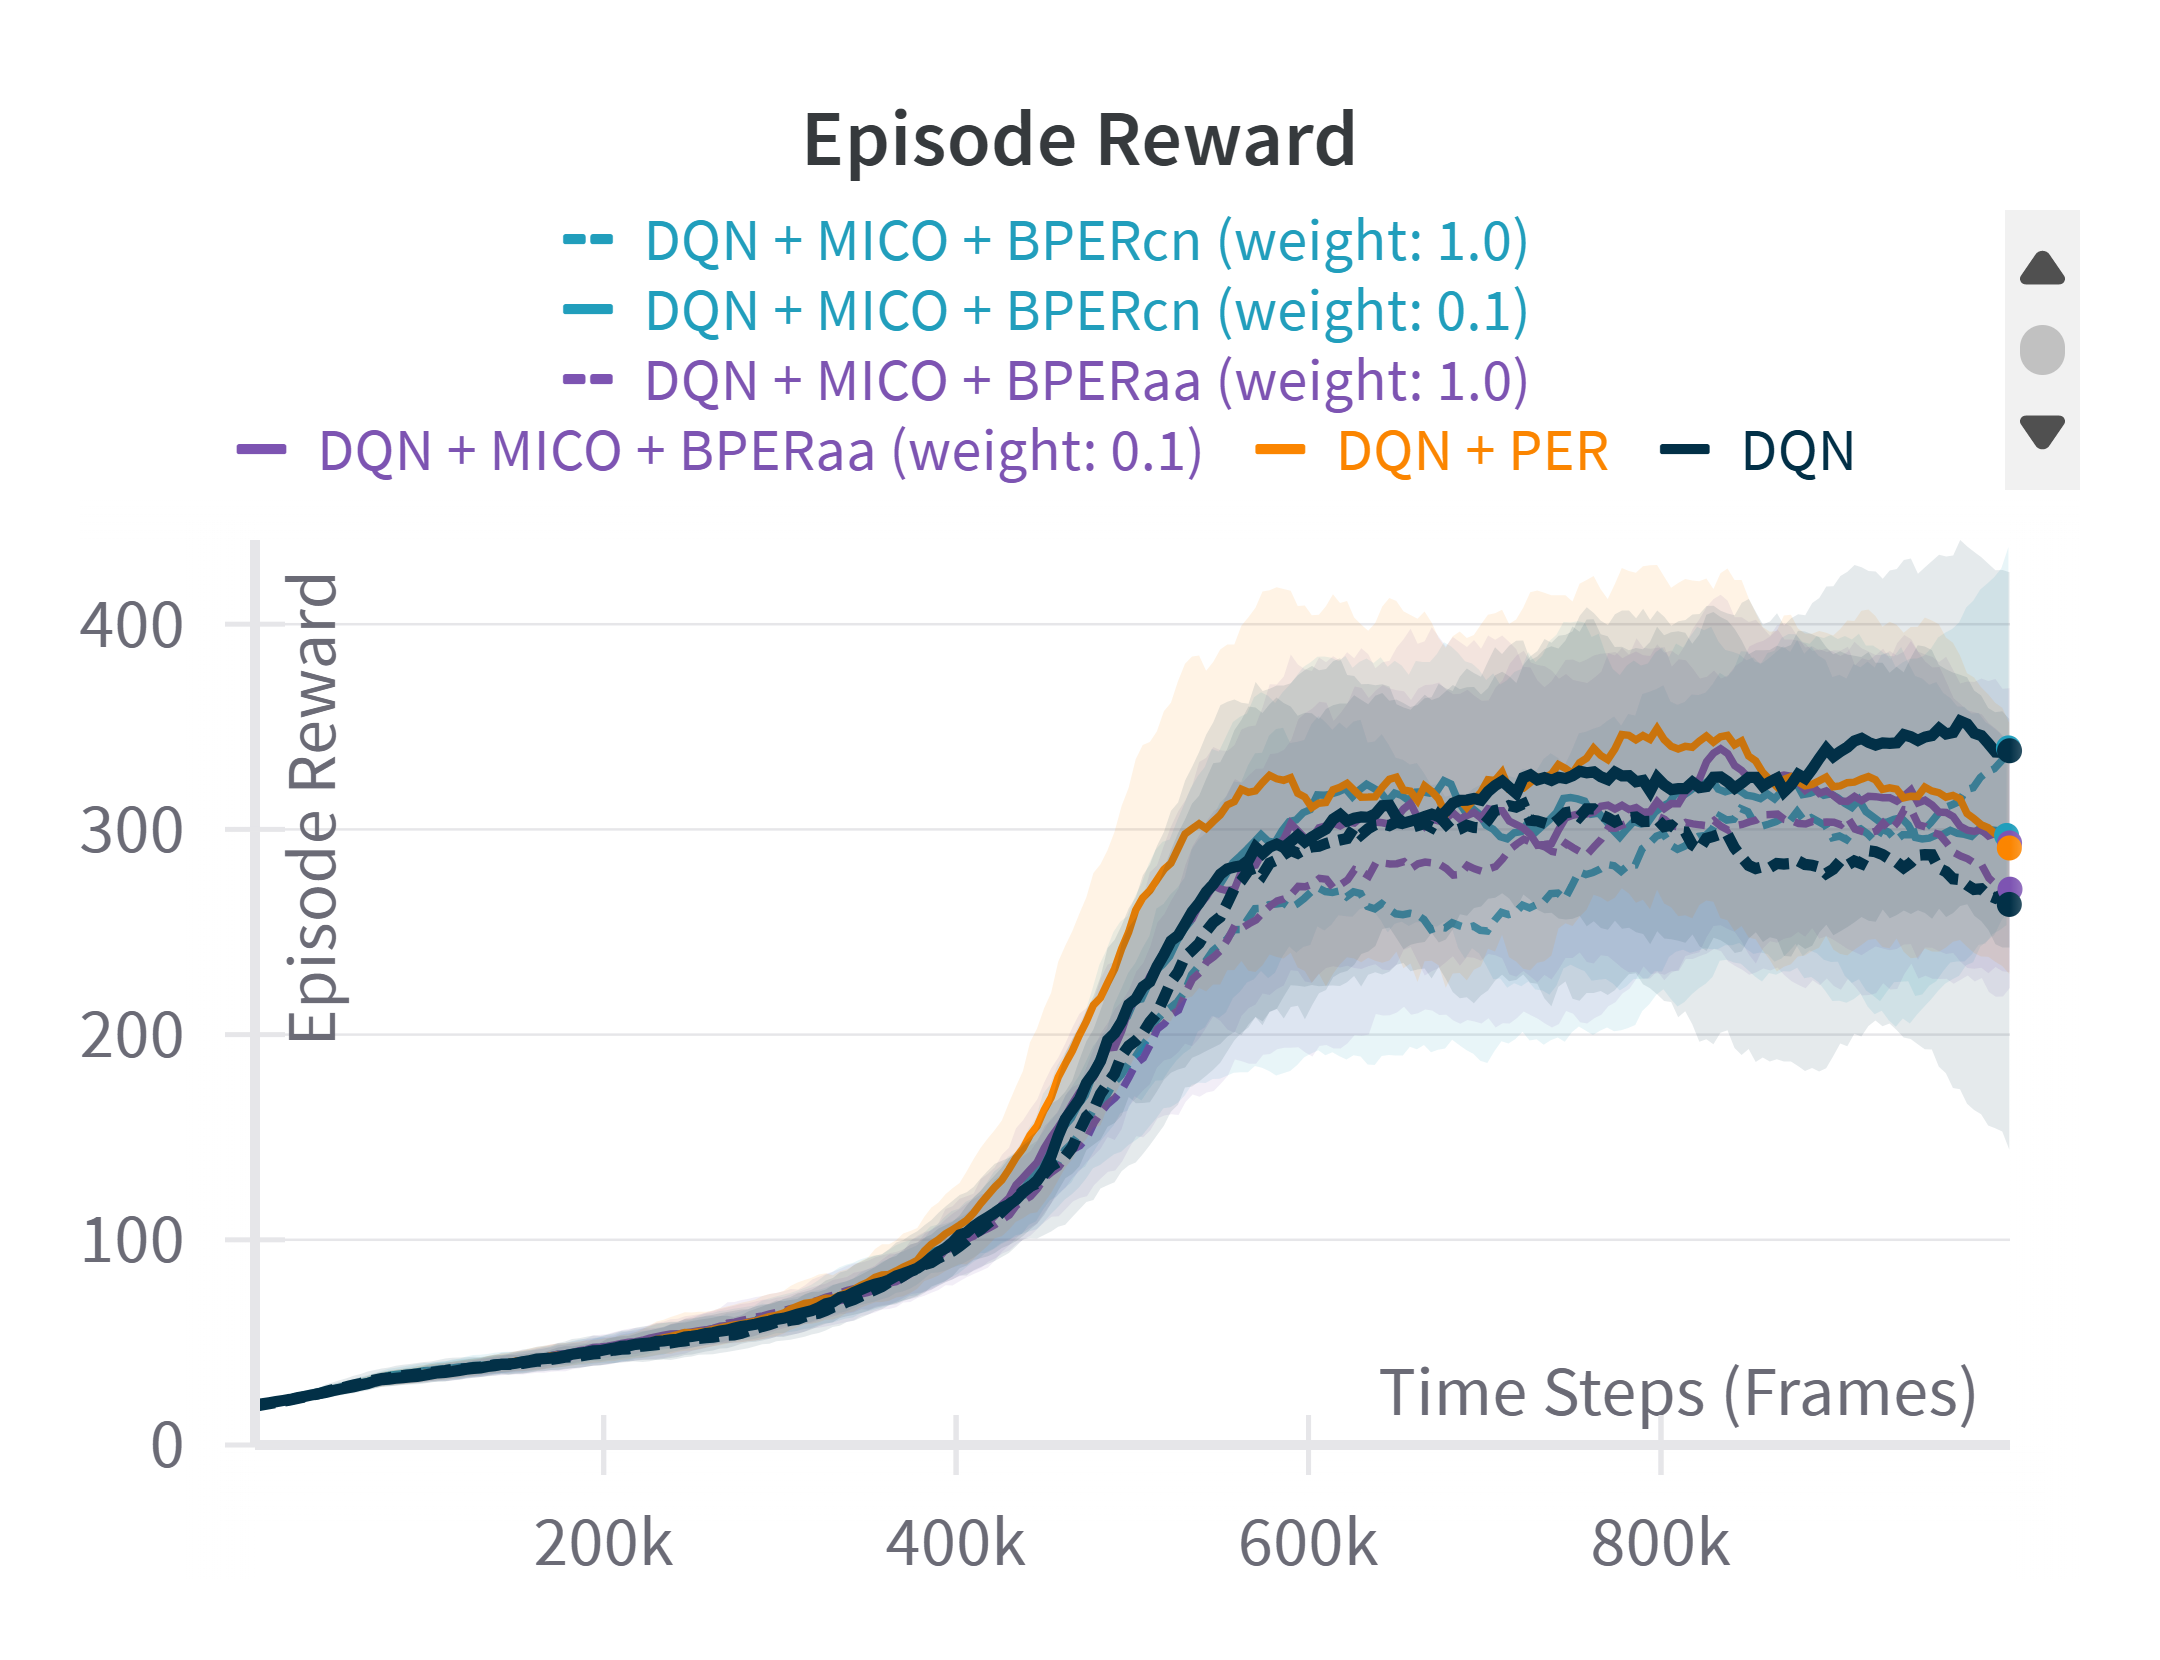
\includegraphics[width=\linewidth]{Results/general_results/return_cartpolev1_weight_1.png}
        \caption{CartPole}
        \label{fig:return_cartpolev1_weight_1}
    \end{subfigure}
    \caption[Episode Reward Priority Weight 1.0]{\textbf{Episode Reward Priority Weight 1.0.} TODO}
    \label{fig:return_methods_weight_1}
\end{figure}

\section{Visual Inspection 50k Time Step}
\label{append:visual_inspection_50k}

\begin{figure}[H]
    \centering
    \begin{subfigure}{1.\textwidth}
    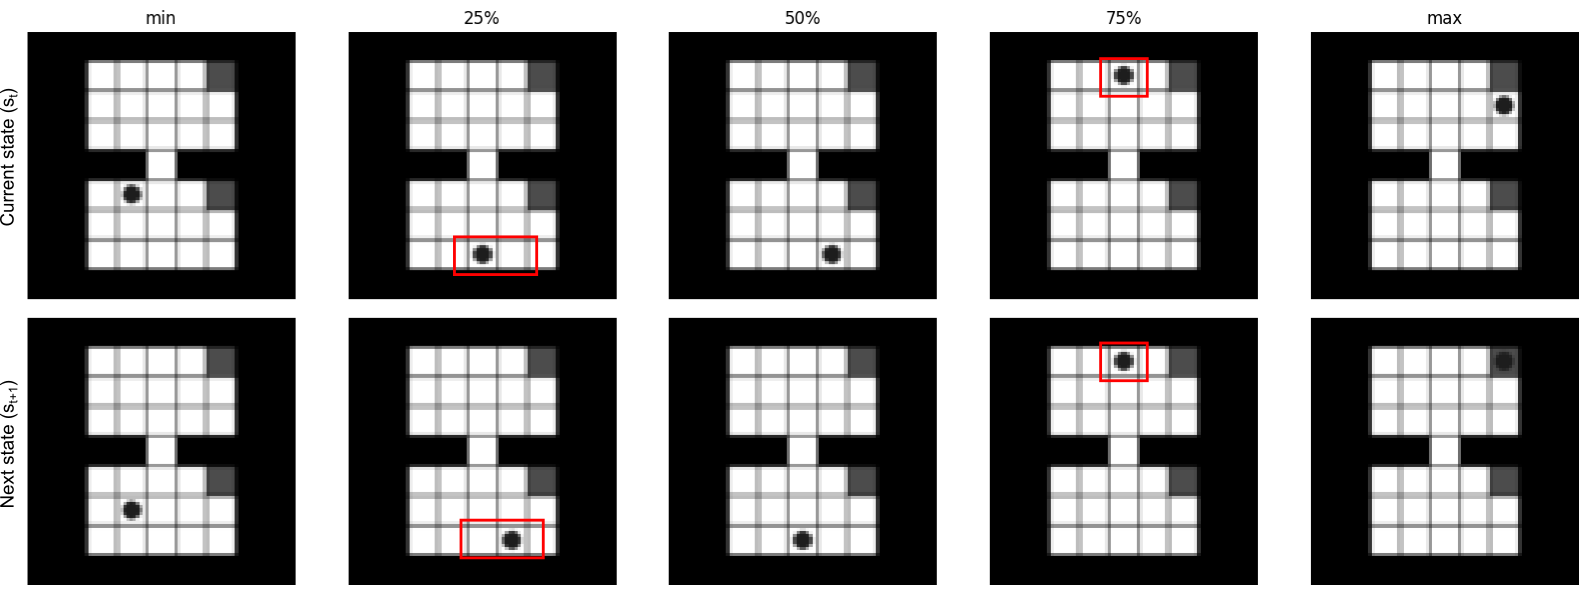
\includegraphics[width=\linewidth]{Results/grid_world/quartiles_images_per_50k.png}
        \caption{DQN + PER}
        \label{fig:quartiles_images_per_50k}
    \end{subfigure}
    \begin{subfigure}{1.\textwidth}
        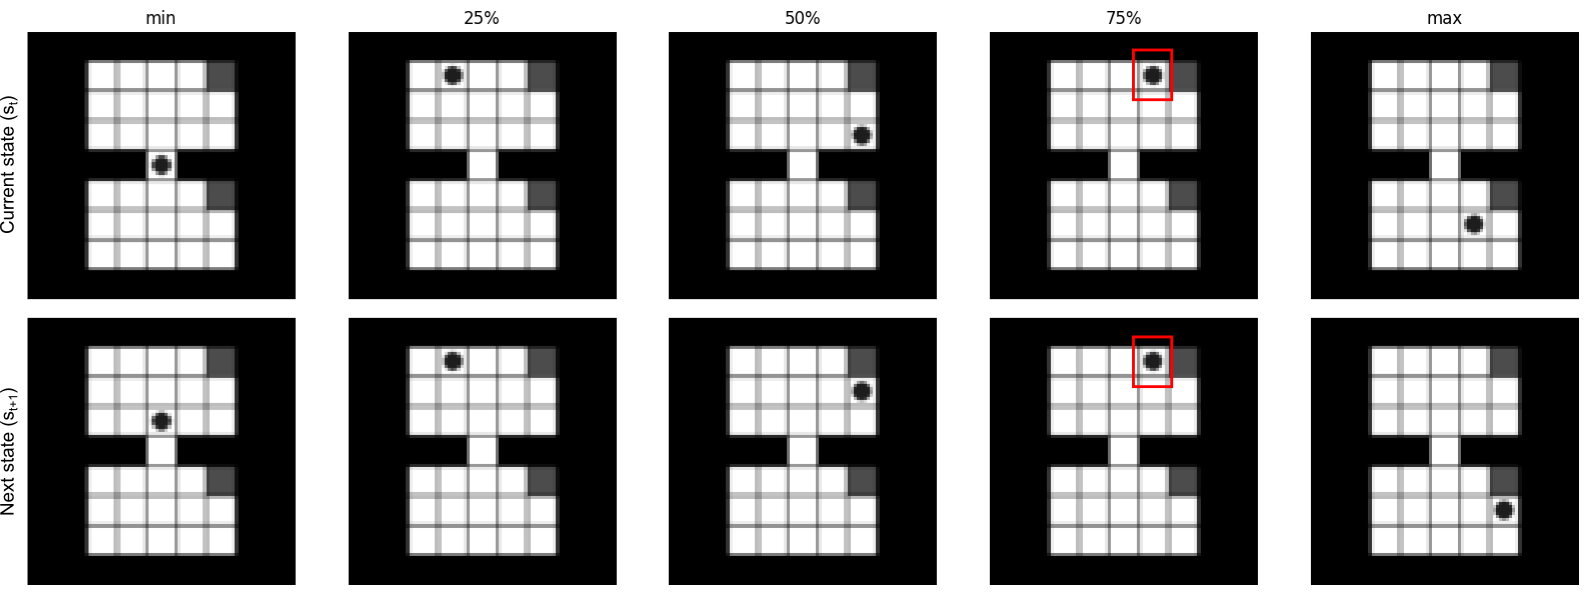
\includegraphics[width=\linewidth]{Results/grid_world/quartiles_images_dqn_mico_bpercn_50k.png}
        \caption{DQN (MICO) + BPERcn}
        \label{fig:quartiles_images_dqn_mico_bpercn_50k}
    \end{subfigure}
    \begin{subfigure}{1.\textwidth}
        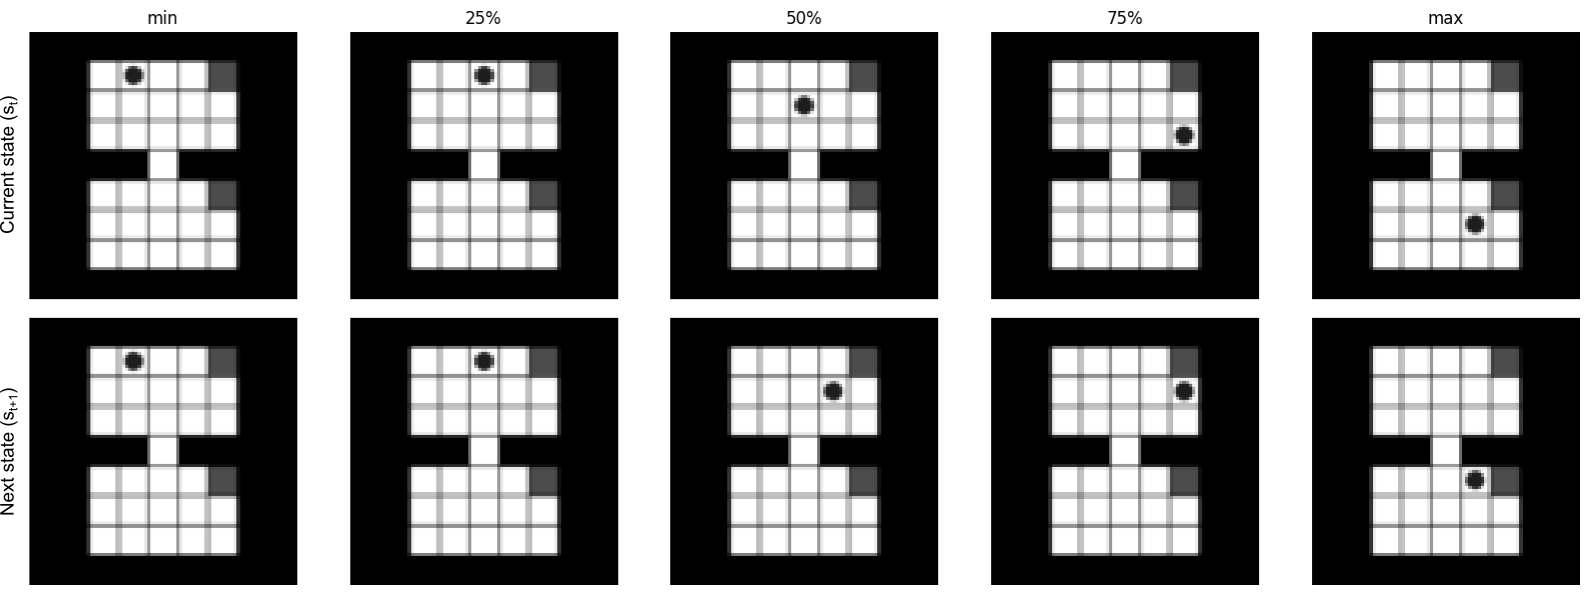
\includegraphics[width=\linewidth]{Results/grid_world/quartiles_images_dqn_mico_bperaa_50k.png}
        \caption{DQN (MICO) + BPERaa}
        \label{fig:quartiles_images_dqn_mico_bperaa_50k}
    \end{subfigure}
    \caption{Two images side-by-side}
    \label{fig:quartiles_all_methods_50k}
\end{figure}

\section{Episode Reward Gain baseline DQN + MICO}
\label{append:episode_reward_gain_dqn_mico}

\begin{figure}[h]
    \centering
    \begin{subfigure}{0.45\textwidth}
    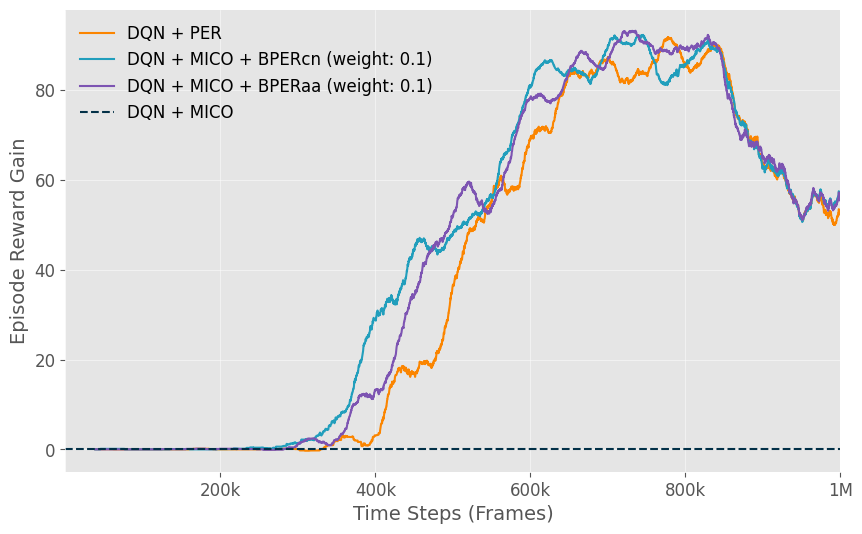
\includegraphics[width=\linewidth]{Results/general_results/mountain_car_reward_gain_vs_dqn_mico.png}
        \caption{MountainCar-v0}
        \label{fig:mountain_car_reward_gain_vs_dqn_mico}
    \end{subfigure}
    \hfill
    \begin{subfigure}{0.45\textwidth}
        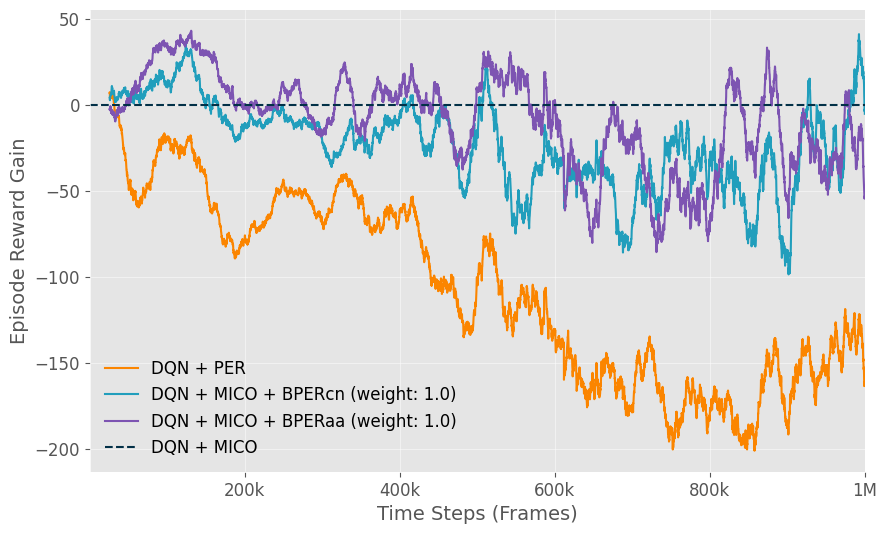
\includegraphics[width=\linewidth]{Results/general_results/lunarlander_reward_gain_vs_dqn_mico.png}
        \caption{LunarLander-v1}
        \label{fig:lunarlander_reward_gain_vs_dqn_mico}
    \end{subfigure}
    \hfill
    \begin{subfigure}{0.45\textwidth}
        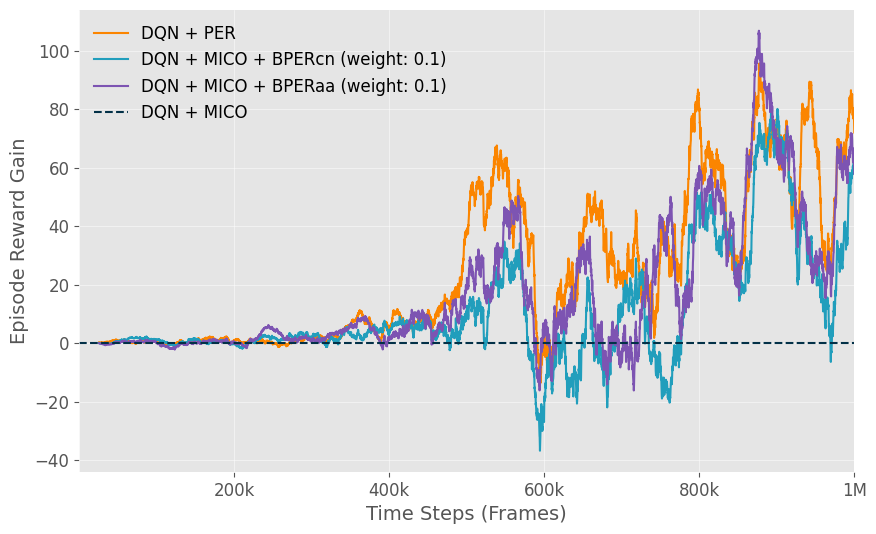
\includegraphics[width=\linewidth]{Results/general_results/cart_polev1_reward_gain_vs_dqn_mico.png}
        \caption{CartPole-v1}
        \label{fig:cart_polev1_reward_gain_vs_dqn_mico}
    \end{subfigure}
    \hfill
    \begin{subfigure}{0.45\textwidth}
        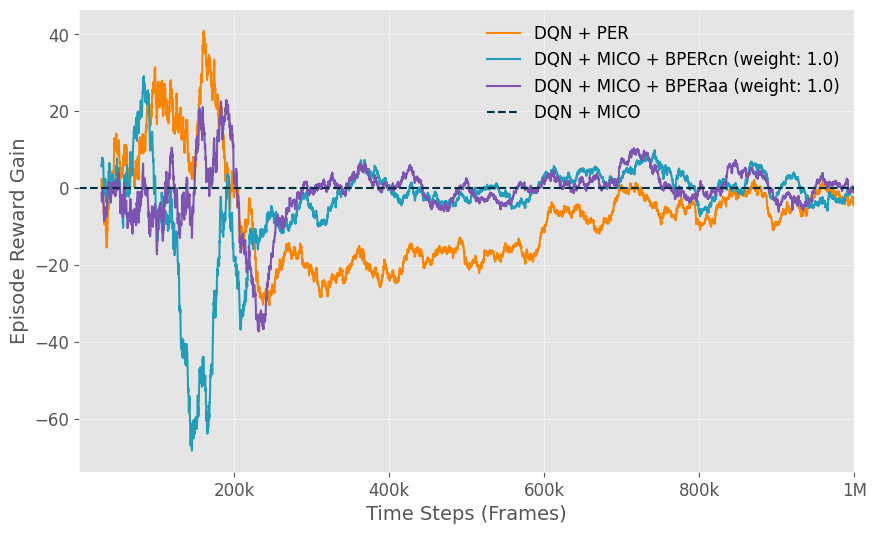
\includegraphics[width=\linewidth]{Results/general_results/acrobotv1_reward_gain_vs_dqn_mico.png}
        \caption{Acrobot-v1}
        \label{fig:acrobotv1_reward_gain_vs_dqn_mico}
    \end{subfigure}
    \caption{Two images side-by-side}
    \label{fig:reward_gain_vs_dqn_mico_methods}
\end{figure}

\section{Cumulative Reward for Lunar Lander}

\begin{figure}[H]
    \centering
    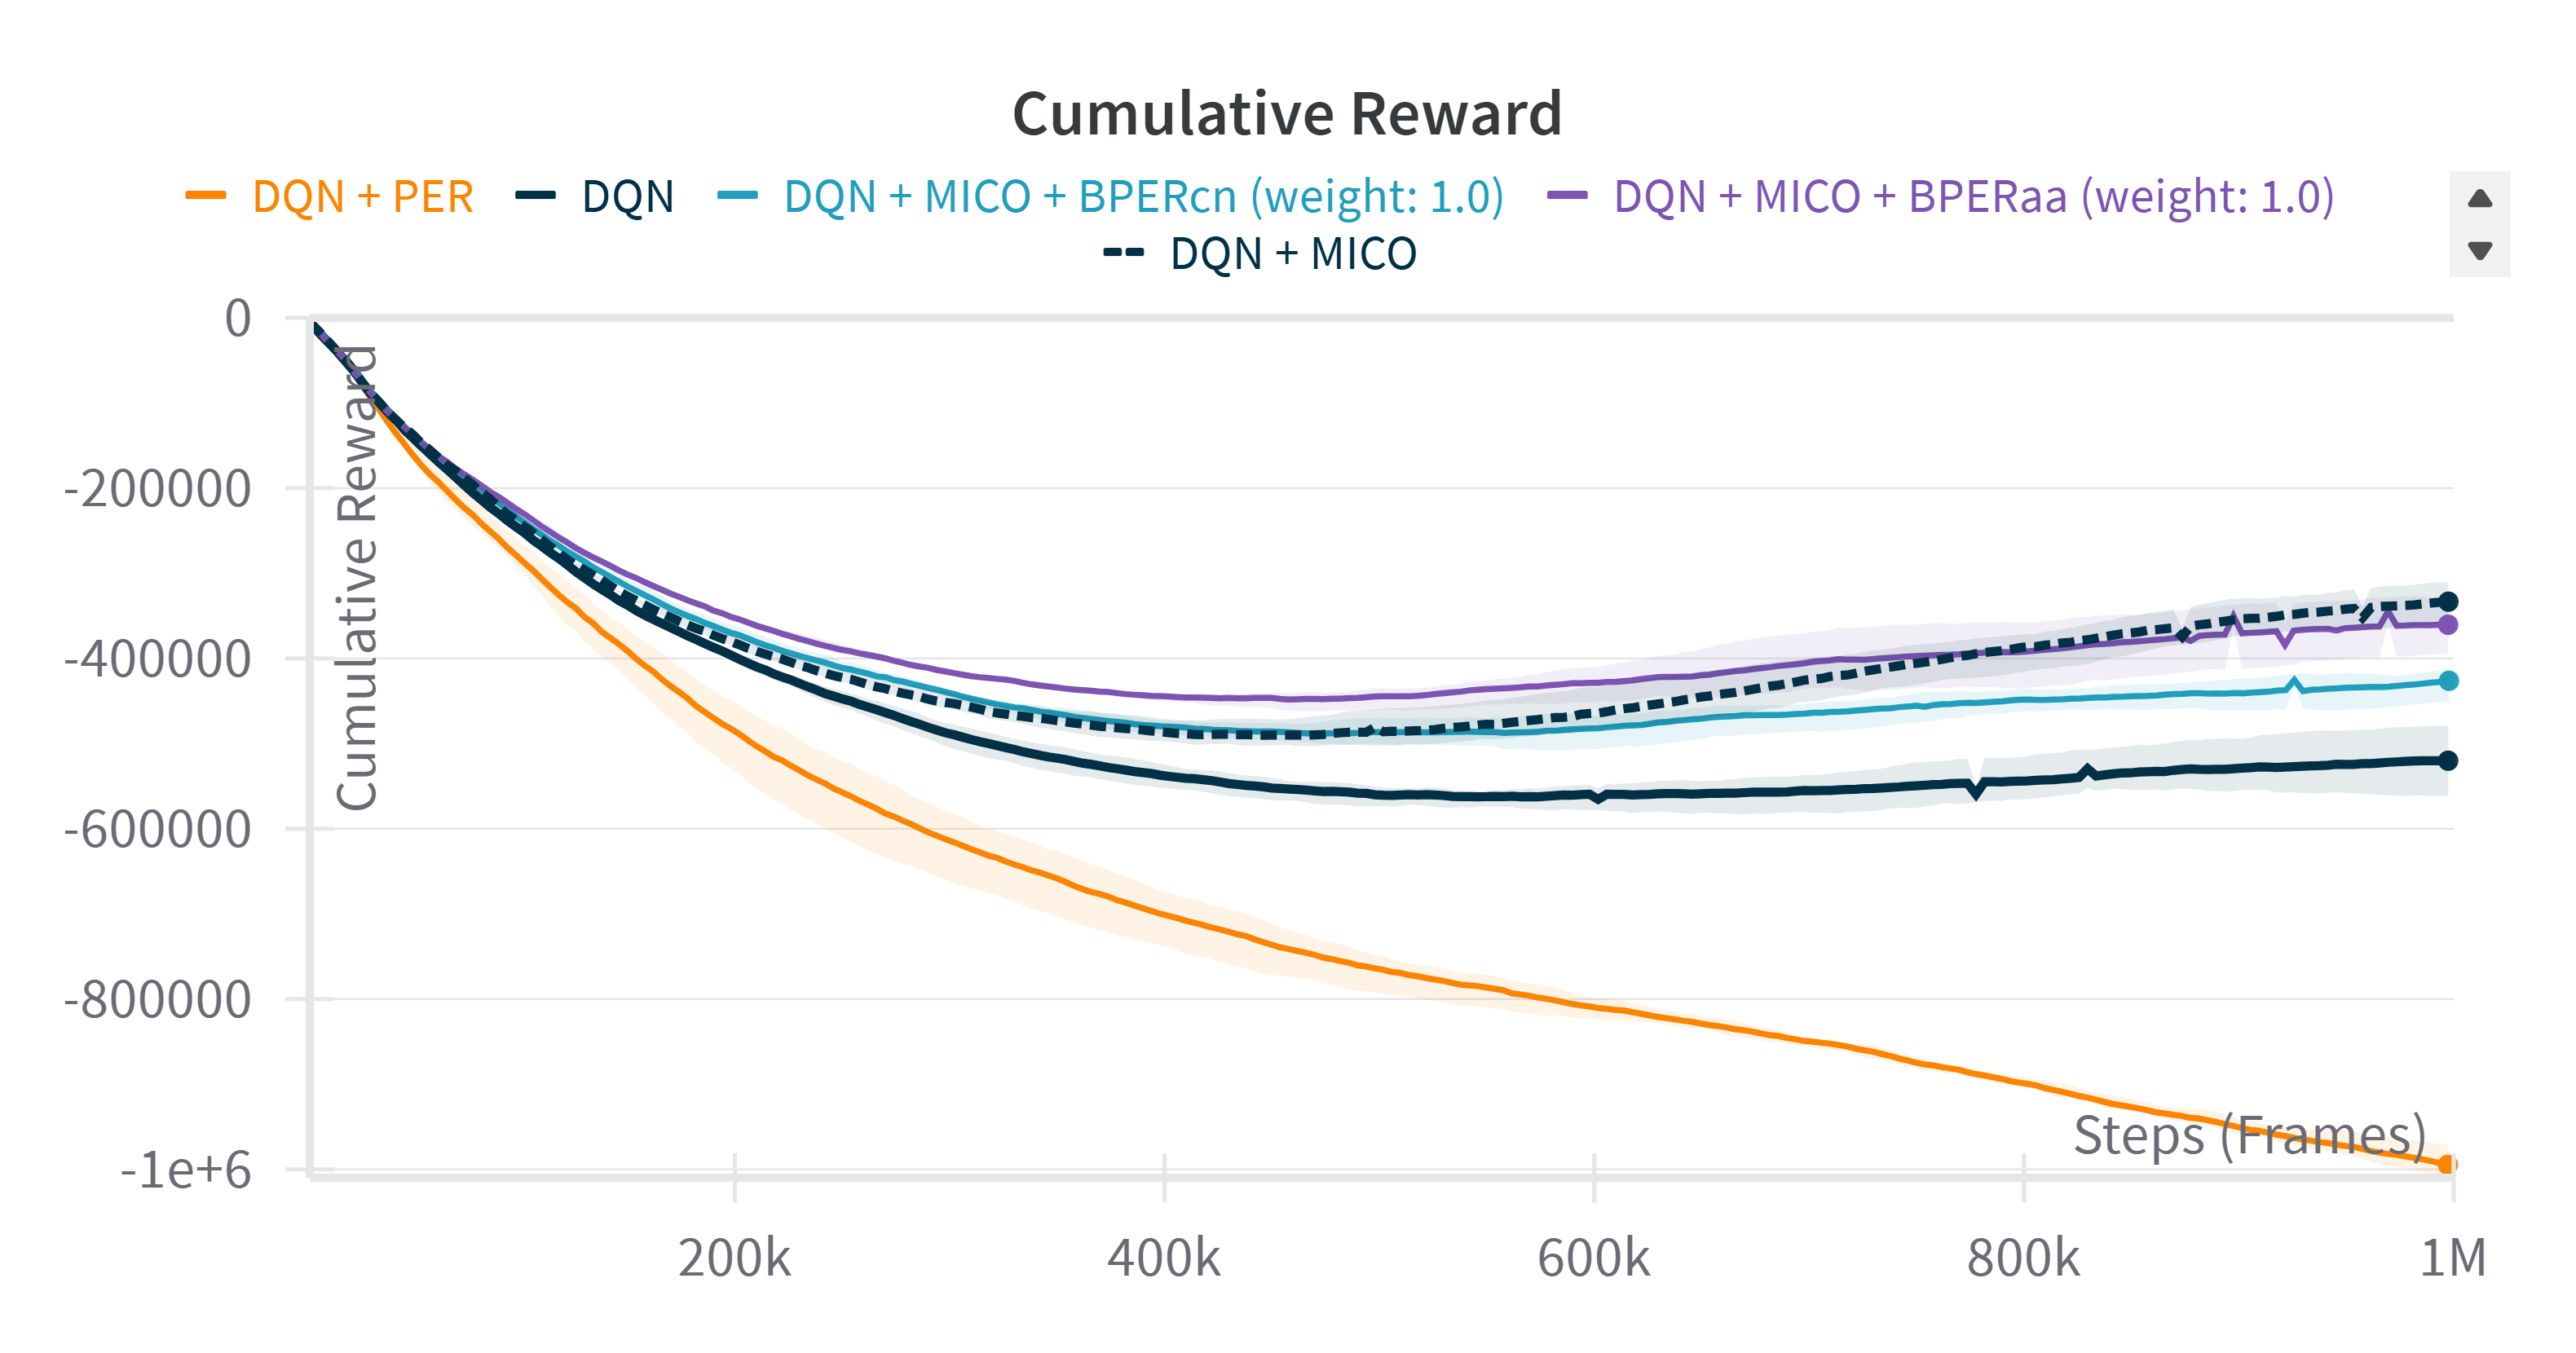
\includegraphics[width=1.\linewidth]{Results/general_results/cumulative_reward_lunar_lander.png}
    \caption[Cumulative Reward for Lunar Lander]{\textbf{Cumulative Reward for Lunar Lander}}
    \label{fig:cumulative_reward_lunar_lander}
\end{figure}

\section{Validation Results}


